\documentclass[letterpaper,10pt]{article}

\usepackage{titling}
\usepackage{listings}
\usepackage{url}
\usepackage{setspace}
\usepackage{subfig}
\usepackage{sectsty}
\usepackage{pdfpages}
\usepackage{colortbl}
\usepackage{multirow}
\usepackage{relsize}
\usepackage{amsmath}
\usepackage{fancyvrb}
\usepackage{amsmath,amssymb,amsthm,graphicx,xspace}
\usepackage[titlenotnumbered,noend,noline]{algorithm2e}
\usepackage[compact]{titlesec}
\usepackage[default]{droidserif}
\usepackage[T1]{fontenc}
\usepackage{tikz}
\usetikzlibrary{arrows,automata,shapes,trees,matrix,chains,scopes,positioning,calc}
\tikzstyle{block} = [rectangle, draw, fill=blue!20, 
    text width=2.5em, text centered, rounded corners, minimum height=2em]
\tikzstyle{bw} = [rectangle, draw, fill=blue!20, 
    text width=4em, text centered, rounded corners, minimum height=2em]

\definecolor{namerow}{cmyk}{.40,.40,.40,.40}
\definecolor{namecol}{cmyk}{.40,.40,.40,.40}

\let\LaTeXtitle\title
\renewcommand{\title}[1]{\LaTeXtitle{\textsf{#1}}}


\newcommand{\handout}[5]{
  \noindent
  \begin{center}
  \framebox{
    \vbox{
      \hbox to 5.78in { {\bf ECE155: Engineering Design with Embedded Systems } \hfill #2 }
      \vspace{4mm}
      \hbox to 5.78in { {\Large \hfill #4  \hfill} }
      \vspace{2mm}
      \hbox to 5.78in { {\em #3 \hfill} }
    }
  }
  \end{center}
  \vspace*{4mm}
}

\newcommand{\lecture}[3]{\handout{#1}{#2}{#3}{Lecture #1}}
\newcommand{\tuple}[1]{\ensuremath{\left\langle #1 \right\rangle}\xspace}

\addtolength{\oddsidemargin}{-1.000in}
\addtolength{\evensidemargin}{-0.500in}
\addtolength{\textwidth}{2.0in}
\addtolength{\topmargin}{-1.000in}
\addtolength{\textheight}{1.75in}
\addtolength{\parskip}{\baselineskip}
\setlength{\parindent}{0in}
\renewcommand{\baselinestretch}{1.5}
\newcommand{\term}{Spring 2014}

\singlespace


\begin{document}

\lecture{ 35 --- Library Card}{\term}{Jeff Zarnett}

In this lecture, we are going to examine three books that cover some important concepts to engineering design. The first is probably the most famous book on software project management \cite{mmm}. The second is a book about how to deal with systems with complex interactions. The content in this section comes from~\cite{lofde} (English translation~\cite{lof}). The third is a book that technically might fall under the umbrella of Systems Design Engineering (SYDE); it is about how to design systems for humans. We spent a lot of time talking about how to design systems, but very little about how to design for people. The content in that section comes from~\cite{thf}.


\section*{The Mythical Man-Month}
Sometimes during development, you might discover that your project is not going well and management might attempt to solve this by adding more resources (workers) to the project. That brings us to one of the most important books in software: the Mythical Man Month~\cite{mmm}. The book is a series of essays, and I feel it would be a very good idea to make sure everyone has some exposure to this before going out into industry. The whole book is worth reading, but we will examine, briefly, two essays from that book.

\subsection*{The Mythical Man-Month}
\begin{quote}
	\textit{Adding manpower to a late software project makes it later.}
\end{quote}

In addition to the standard problem that estimates are difficult to make and usually optimistic, our estimating techniques tend to confuse effort with progress, assuming that programmers and months are interchangeable. When a schedule slip is recognized, the natural tendency of management is to add more programmers to the team. This is like trying to douse a fire with gasoline: it makes the problem worse, and can lead to a spiral where adding more programmers causes a need for more programmers...

A \textit{man-month} is defined as the amount of work one programmer can accomplish in one calendar month. Cost varies by programmers and months, but progress does not. It is therefore dangerous and wrong to try to measure a programming task using this unit.

Workers and time can be traded off against one another for tasks only if there is no communication required between workers. (Does this sound familiar? We talked about this in the lecture about multithreading). This is not true of programming. When more programmers are added, we have to consider training and intercommunication.

Training scales linearly ($n$) with the number of people. Training consists of bringing a new programmer up to speed on the project and its related technology. This is a one-time cost when someone joins a project, but it means a new programmer, no matter how intelligent, is not fully productive immediately.

Intercommunication scales at $n (n - 1) / 2$, if each part of the task is separately co-ordinated with each other part (worst case scenario). Three workers require three times as much intercommunication as two; four require six times as much as two. Beyond a small number of programmers, adding an additional programmer increases the communication costs so much that it outweighs the benefit the additional programmer brings in ability to accomplish work. Thus, adding a new programmer to the team makes the project later.

Suppose a task is estimated at 12 man-months: and it is divided up such that three are three programmers who will work for four months. There are milestones A, B, C, and D, one at the end of each month. 

A delay occurs and milestone A is not completed in one month; it takes two months instead. Management would still like this to be completed in four months (total) and they think that the solution is to add some additional programmers. They assume that only milestone A is incorrect and 9 man-months of work remain, and two months remain. So 4.5 programmers will be needed. Add two programmers. 

Let's assume it takes one month to train these two new programmers. So now in addition to having had milestone A take longer, developer time is consumed with training the new people. Also the tasks must be re-partitioned and re-assigned, and because there are more people working on different parts, more integration testing will be needed to deal with the bugs caused by the interaction of modules written by different people with slightly different assumptions. At the end of the third month, we would still have more than 7 man-months of work to do and five trained programmers. The project is still late! The temptation is to then add yet more people, but this makes things worse, not better. 

\subsection*{No Silver Bullet}
\begin{quote}
\textit{There is no single development, in either technology or in management technique, that by itself promises even one order-of-magnitude improvement in productivity, in reliability, in simplicity.}
\end{quote}

The term ``silver bullet'' comes from the folklore of werewolves -- humans who supposedly transform into giant wolves when the moon is full. Werewolves can be stopped by being shot with a silver bullet (regular ones apparently do not work). The term (or sometimes, magic bullet) is a metaphor meaning a straightforward, simple solution to what is otherwise a complex problem. For a non-programming, non-computer related example, diet books often promise something extremely simple as the solution to weight loss, as if all one has to do is eat Goji Berries. It is, unfortunately, not that simple. The essay ``No Silver Bullet'' is actually not in the original edition of the Mythical Man-Month book; see~\cite{nsb}.

It is unlikely, given the nature of software, that we will ever find a silver bullet; there are probably no inventions that will do for software development what electronics, transistors, and VLSI (very large scale integration) did for computer hardware. The hard part of building software is not the accidental complexity, but the essential complexity; the hard part is the specification and design of testing the concepts, not the work of implementing it. 

Software is very complex, and this is an essential property. Math and physics experts can create simplified models for complex phenomena (e.g., Newton's equations). Complexities (like relativity) can be ignored. In software, the complexity, the details, are the essential parts and cannot be abstracted away. Much of the complexity is arbitrary, unfortunately, because it must conform to other software or hardware, designed by imperfect humans. Your software has to run on Microsoft Windows, for example, and has to conform to all the details and oddities of Windows...

Similarly, software is much more changeable than physical objects. Cars and buildings get upgrades infrequently if ever. If Ford comes up with a better version of a car, that goes into next year's model. Software is changeable precisely because it is not a physical artifact; buildings get changed infrequently and the fact that the cost of change is high discourages arbitrary changes. Successful software is changed because users want to apply it to new problems or because new hardware or operating systems are released and the software has to be adapted to it.

Our tools have improved to make attacking some of this complexity better, but none alone is the magic solution: high-level languages, integrated development environments, object-oriented programming, verification. Some breakthroughs have been promised for a long time, but never seem to come through: artificial intelligence, ``automatic programming'' (where the code is generated based on the problem definition), and graphical programming. Maybe these things will arrive at some point, but we are still waiting. The most powerful tool we have is to have great developers (...which is one reason why you are here in this class).



\section*{The Logic of Failure}

Tanaland is a fictional region in West Africa, inhabited by fictional nomadic herders who hunt and raise fictional cattle and sheep, as well as some farming communities. It is used as the setting of a simulation where participants in the study get dictatorial power and the goal of improving the lives of the inhabitants over a period of ten years. 

For example, in Tanaland, the fields are not very productive, partly because of the rodents (mice, rats, etc.). The obvious solution is to exterminate the pests. At first, this results in an increase in the productivity of the fields as desired. Then, insect populations increase (because they also feed on the fields), and larger predators begin attacking the cattle since there are no longer the mice and rats to feed on. It is possible that eliminating the rodents in the end has no effect, or it may have actually made the situation worse. The critical insight from the simulations is that we cannot do any one thing in isolation: any change has multiple effects.

\textit{Positive Feedback} in a system means an increase in one variable produces a further increase in that variable; a decrease produces a further decrease. Animal populations in isolation, for example, experience positive feedback: if there are more rabbits, they have more babies, producing yet more rabbits, who will in turn have more babies... Positive feedback is inherently unstable and can easily lead to disaster.

\textit{Negative Feedback} in a system is the opposite: an increase in one variable produces a decrease in another and vice versa. This maintains equilibrium. Predator-prey relationships in nature are an example. An increase in the prey population will produce an increase in the predator population; the increase in the predator population results in a decrease in the prey population, and the decrease in the prey population then leads to a decrease in the predator population. Over time, the predator and prey populations tend towards a stable range.

Let's examine the concept of feedback, using some examples and images from~\cite{hackerdiet}. In a system where the relevant variable is temperature, let's assume we have a thermometer (which, for some reason, measures things in Fahrenheit rather than a sensible metric unit):
\begin{center}
	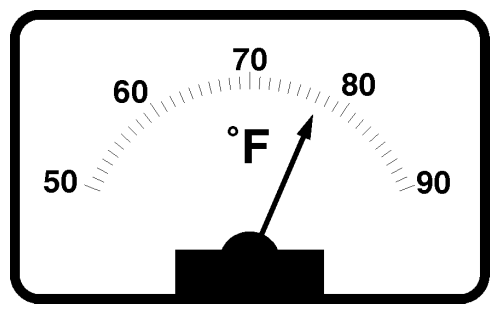
\includegraphics[width=0.4\textwidth]{images/thermometer.png}
\end{center}

And imagine that the temperature varies as follows:

\begin{center}
	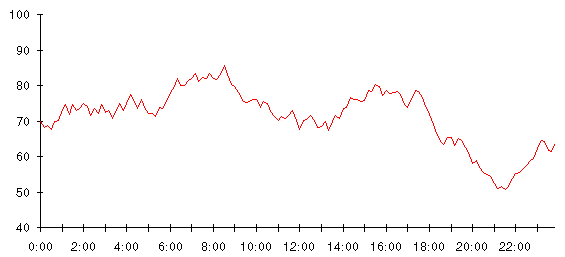
\includegraphics[width=0.4\textwidth]{images/temperature-chart.png}
\end{center}

This system has no feedback mechanisms. Our situation looks something like this:
\begin{center}
	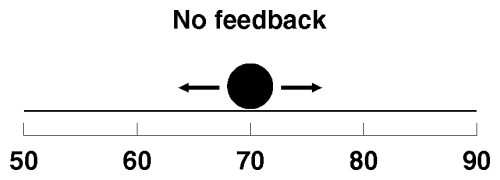
\includegraphics[width=0.4\textwidth]{images/nofeedback.png}
\end{center}

The ball can move freely in either direction and its movement is not resisted. Suppose, however, we have a concept of too hot and too cold:
\begin{center}
	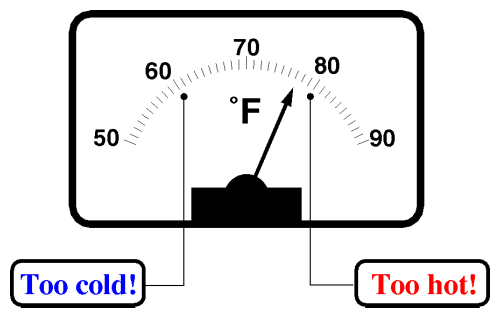
\includegraphics[width=0.4\textwidth]{images/temperature-hotcold.png}
\end{center}

Representing these limits on the temperature chart, we see:

\begin{center}
	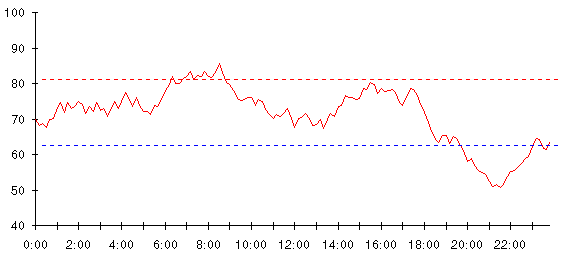
\includegraphics[width=0.4\textwidth]{images/temperature-chart-hotcold.png}
\end{center}

Let's set up a negative feedback system:
\begin{center}
	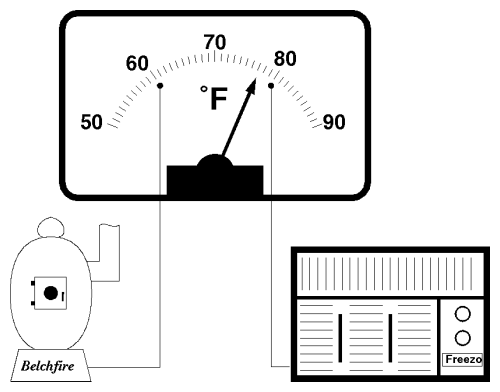
\includegraphics[width=0.4\textwidth]{images/negativefeedbacksystem.png}
\end{center}

When the temperature gets too cold, the Belchfire heater activates to warm the place up; when the temperature gets too high, the Freeze air conditioner activates to cool things down. Within the acceptable range, there is no resistance to movement, but when things are moving outside of that range, the system moves it back towards the middle.

\begin{center}
	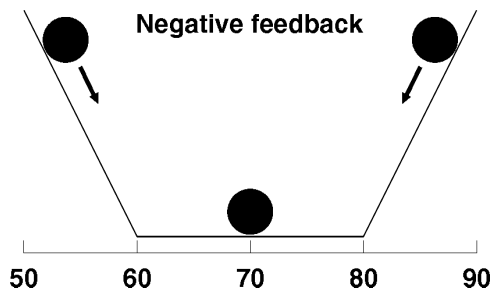
\includegraphics[width=0.4\textwidth]{images/negativefeedback.png}
\end{center}

But, what if we hooked it up backwards? Now when it is too hot, the heater activates to make things even warmer.

\begin{center}
	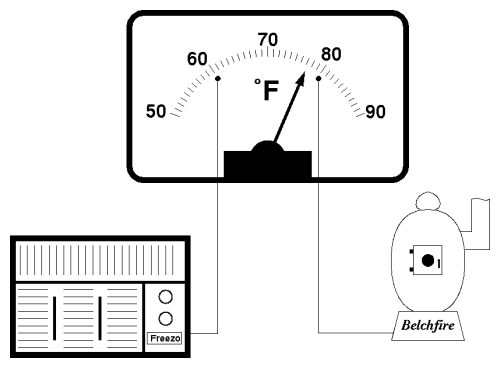
\includegraphics[width=0.4\textwidth]{images/backwardssystem.png}
\end{center}

This results in a positive feedback system:

\begin{center}
	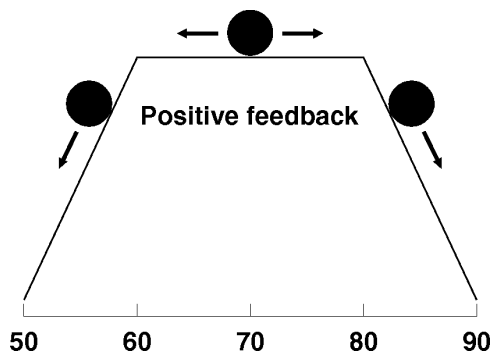
\includegraphics[width=0.4\textwidth]{images/positivefeedback.png}
\end{center}

Within a certain range things seem fairly stable... but pushed too far in one direction or another, the system falls off a (figurative) cliff!


A \textit{Well-Buffered System} incorporates many variables regulated by negative feedback. It can absorb many disturbances without becoming unstable. However, buffers are limited and may eventually be exhausted. If the predator population is excessively large it can hunt the prey to extinction.

\textit{Critical Variables} are those that interact with a large number of other variables. Altering a critical variable has a major impact on the state of the system.

\textit{Indicator Variables} depend on many other variables but themselves exert very little influence. These help understanding of what the current status of the system is. 

\paragraph{Conflicting Goals.}
In complex situations, we can rarely focus on one goal at a time. If analysis shows that shopping options and transportation links in a suburb are inadequate, we can choose to improve one of these, but choosing one will have an impact on the other. If we improve transportation, people might drive into the city and shop there, depriving local shops of revenue (or people from the city will come shop in the suburbs -- it's hard to know which!). If we improve local shopping opportunities, but transport remains inadequate, then people will shop locally and things will improve for local businesses. 

The relationship still exists even if there are no complaints about shopping. If we improved transport, it might ruin or improve things for the local businesses even if we did not realize they were related.

By solving problem $X$ we create problem $Y$. If the appearance of $Y$ is not immediate, it might not be obvious that solving $X$ was the cause. Solving $Y$ could very well result in a recurrence of $X$, starting the cycle all over again. Someone with a headache might take some medicine that cures the headache but will give him a stomachache tomorrow. The pain of the headache is real and the stomachache is an abstraction, and in the future, and not a certainty anyway. And yet, on the next day, when he does have a stomachache, he would take another medicine to relieve the stomachache even if its side effect is that on the next day, he would suffer a headache...

\subsection*{The Plight of the Moros of Tanaland}
We will examine in more detail the plight of a group of nomadic inhabitants of Tanaland, the Moros. The approach that most people take to address their problems is to solve one problem at a time.  The problem most people start with is combating the Tsetse fly, a parasite  that attacks cattle. The next biggest thing is to drill wells to alleviate a water shortage.

So far this seems good: the Moros' water shortage is eased and they can have bigger fields of grass and more cattle. They can sell some grain and cattle, and they had some extra money. The next step most people take is to address medical care, so infant mortality declines and life expectancy increases. This results in an increase in population. This can go three ways, but all of them end in the same (grim) way.

\paragraph{1. Cattle Catastrophe.} The number of cattle exceeds the carrying capacity of the fields. The cattle are not only eating the grass, but tearing it up. The vegetated area is overgrazed and shrinks. The smaller the amount of grass, the more desperate the hunger of the cattle and the more they damage the grass (positive feedback). There is a way out of this -- slaughter or sell the majority of the cows -- but this seems like a ``radical'' step and people are reluctant to do it. Once the grass is gone, the cattle will die, the Moros will be short of food, and they will starve.

\begin{center}
	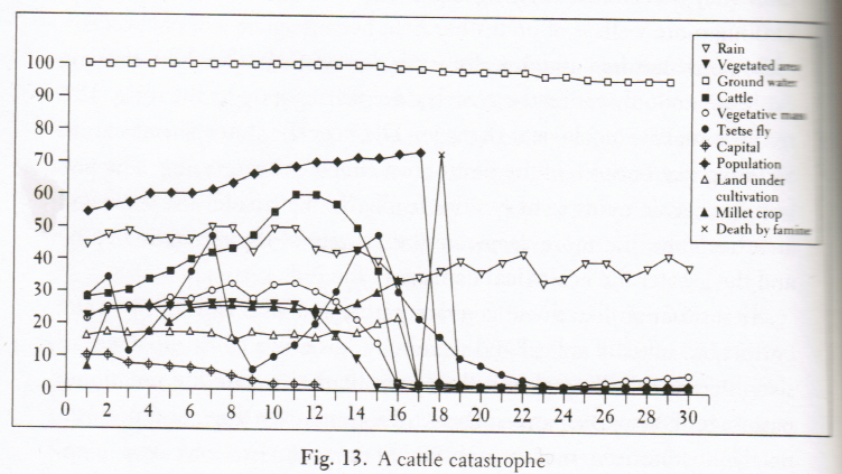
\includegraphics[width=0.8\textwidth]{images/cattlecatastrophe.png}
\end{center}

\paragraph{2. Groundwater Catastrophe.}
Some people were cautious with the cattle and keep the herds at an appropriate level. If they keep population under control, the system might be stable for some time. At some point, however, the wells start yielding less water. The obvious solution is to drill more wells. It is easy to interpret this as just a temporary variation, perhaps because rainfall was slightly lower in one year than another. But the groundwater supply is being depleted all the same and soon the wells are practically dry. Drilling new wells in the face of depleted wells is a positive feedback loop: the more wells there are, the faster the groundwater is depleted. The shortage of water means no irrigation of the grass. And this means the situation starts to look like scenario 1: the cattle start overgrazing, then die, the Moros are short of food, and starvation occurs.

\paragraph{3. Population Catastrophe.}
Another participant just focused on health care: improving the lives of the Moros in small ways. But as infant mortality decreases, and life expectancy increases, the population grows. More people means more requirements for food and water. If nothing is done, a famine will occur. Trying to take steps to increase cattle or groundwater can easily degenerate into scenario 1 or 2.

\paragraph{Conclusion.}
All catastrophic outcomes came about because the participants in the study dealt with things as independent mini-systems and not a single, complex, interrelated system. They focus on the problem at hand (``we need more water for the cattle'') and not what the consequences are or could be. Future problems don't seem important because the current problems are pressing. Furthermore, the cause-effect relationships are unclear and are at best revealed by experimentation.

\subsection*{Lessons Learned}

Good participants asked more why-questions as opposed to what-questions. They were more interested in how the events were interrelated; people who did poorly tended to take events at face value and not dig as deep into the situation.


\paragraph{Tips.}
 Some tips for dealing with complex systems:

\begin{itemize}
	\item State goals clearly.
	\item Recognize that it's not always possible to accomplish all our goals at once (goals may conflict).
	\item Establish priorities and change them when circumstances require.
	\item Learn a model of the system and use it to predict likely outcomes.
	\item Gather information at an appropriate level: neither too much nor too little.
	\item Know when to gather more information and when enough. 
	\item Avoid excessive abstraction.
	\item Don't hastily blame all events on one central cause.
	\item Avoid ``knee-jerk'' reactions.
	\item Analyze errors and learn from them.

\end{itemize}

\section*{The Human Factor}
In the Mercedes-Benz E320, drivers can check the oil electronically from the driver's seat. The ``normal'' procedure is open the hood, find a rag to wipe the dipstick, identify the dipstick, lift the dipstick, wipe it, reinsert it, extract it and read it. What an advance to be able to do it electronically. What are the steps?

\begin{enumerate}
	\item Turn the car off.
	\item Wait for the oil to settle. (So far, normal.)
	\item Turn the ignition two notches to the right. (Unusual, but... okay.)
	\item Wait five seconds. (why five seconds?)
	\item Press the odometer reset button twice. (What?!)
\end{enumerate}

Will users remember these set of steps? Probably not: most people will just perform the manual procedure. Designers didn't deliberately build this system to be complicated and unintuitive. They didn't sit around laughing maliciously about how they could choose the strangest series of steps to confound the drivers. At least, as far as I know.

We, the designers of systems, are responsible (but not maliciously). We like playing with gadgets and figuring out the cool features of something. Most people, however, just want to use whatever they are working with and don't really care. We have to consider that most users are not like the designers. Sticking with the car example, the 2003 BMW 7 series had an electronic system called electronic dashboard system called iDrive. This product had somewhere between 700 and 800 features, and Car and Driver magazine called it ``a lunatic attempt to replace intuitive controls with overwrought silicon''. Road \& Track magazine hit the nail on the head: ``It reminds me of software designers who become so familiar with the workings of their products that they forget actual customers at some point will have to learn how to use them.''

When designers make completely unrealistic assumptions about physical systems or processes, they are blamed for technical incompetence. Yet, when they make incorrect assumptions about human nature or performance, like making sense of 800 features in a car, we don't blame the designers, we often blame the users.




\subsection*{``Human Error''}
\begin{quote}
\textit{Physicians are expected to function without error, an expectation that physicians translate into the need to be infallible. One result is that physicians... come to view an error as a failure of character -- you weren't careful enough, you didn't try hard enough... the perfectibility model: if physicians could be properly trained and motivated, then they would make no mistakes.}
\end{quote}
\hfill - Lucian Leape

Research on patient safety unambiguously shows that in most cases where patients are injured or killed are the result of honest mistakes by otherwise good medical practitioners. Expecting them to be perfect is not going to happen. Human nature is to find a culprit and blame that person. The remedy is in design: create better systems to make it harder to make a mistake and easier to do the right thing.

Changing tracks, an airplane example. In 1943, pilots of several kinds of US aircraft, (B-17s, B-25s, P-47s) frequently retracted the landing gear wheels rather than the flaps\footnote{Aviation lesson: flaps are used to change the aerodynamic characteristics of the wings by extending or retracting to make the wing larger or smaller in different dimensions.}. Pulling up the wheels when the plane is on the ground is bad for the plane. The problem is not just limited to new, inexperienced pilots. The military considered this ``pilot error'', but they investigated the matter.

Their investigator, Alphonse Chapanis, determined that the levers controlling the landing gear and the flaps were next to each other and very similar in appearance. On a different plane, the C-47, they weren't next to each other and operated differently. Unsurprisingly, the C-47 did not suffer from landing gear accidents. Moving the controls was not realistic on already-built, in-use airplanes. As the short-term fix, Chapanis added a small wedge-shaped end to the flap controls and a small rubber disk to the wheel control. There was now a clear relationship between the controls and their function (wheels are round and made of rubber; flaps are metallic and wedge-shaped), but most importantly, the controls were different. If a pilot touched the wrong one, it was immediately obvious. Pilots using the new design stopped retracting their wheels while on the ground.


\subsection*{Designing with Humans in Mind}
At the lowest level, when we design for humans, we should respect what human bodies are like. Asking operators to read a dial located 4 metres off the ground is difficult. Similarly, expecting people to lift 1000 kg unaided is not realistic. As an example, consider a lathe, a device used to machine metal parts. A study of the device under normal operation would reveal what dimensions a person would have to have to use the machine optimally. A study conducted by Patrick Foley on one such lathe revealed that the ideal user would be 130 cm tall, with shoulders 60 cm wide, and an arm span of 243 cm. In other words, a very strange looking alien. Somehow, machinists cope with using this lathe, probably by moving around and contorting themselves a lot. 

Even if a design is a good fit in physical terms, we also need to consider the psychological perspective. Some relevant criteria include the length of human short- and long-term memories, the limited ability to perform mental calculations, and basic expectations. Turning the steering wheel to the left should make the car go to the left; if it goes to the right it confounds our expectations for how it should behave. The difficulties we encounter with computers are very often psychological: users can click the mouse and type with the keyboard, but getting the computer to do what the user wants is more difficult: remember the command, or navigate the menu.

\paragraph{Example: The Four Burners Problem.}
In the four burner problem, we take a typical stove top and see four burners on it. Then we have four knobs to control each of those burners. The burners are arranged in a square formation, one in each quadrant of the stove top. The controls, however, are in a linear sequence. So the question is, which knobs control which burners?

Often there is a little diagram highlighting which of the burners a knob applies to. This is a start, but even with that people sometimes turn on the wrong burner. If you turn on the wrong one it might just be embarrassing, but there's also the possibility of damaging a kettle or accidentally starting a fire. 

Solution: lay out the burners in a more intuitive way. Consider the graphic below; compare the top representation (standard quadrant arrangement) with the bottom representation. On which of these is an error more likely to occur?
\vspace{-0.5em}
\begin{center}
	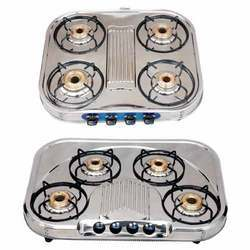
\includegraphics{images/4-burner.jpg}\\ \texttt{http://www.indiamart.com/kitchentech/four-burner-stove.html}
\end{center}

\paragraph{Make Errors Impossible.}
Designing objects can be done in such a way that errors are eliminated. Why are USB plugs really annoying? The first way you try to plug it in doesn't work, then you flip it over, and it still doesn't work, so you flip it back again and somehow it works this time. The USB group finally figured it out when they announced their type C connector is reversible: there is no ``wrong'' way to plug it in; both ways work. Another example is a laptop battery: its asymmetrical shape and notches mean it can fit into the laptop computer in exactly one orientation.

\paragraph{Feedback.}
Humans respond really well to feedback. If there is a campfire, up to a certain point, getting nearer to the campfire is nice. If you try to get too close, the temperature increases until it feels uncomfortable, and if you get really close it can get painful. When you step away, the temperature decreases. It's very obvious what the effect of taking a step in a particular direction (towards/away) is. Note that there are also warning signs (uncomfortable temperature, or mild pain) that warn you of the danger of being too close to the fire (getting burned).

Lack of feedback is the cause of many errors (big and small). For example, my grandmother's flat screen TV. When you press the power on the remote, it takes a few seconds before any indication appears on the TV that it's powering on (a little LED comes on). The result is that for the first few seconds, I don't know if I pressed the power button while the remote had proper line of sight to the receiver successfully or not. If it was but I think it wasn't, I press the button again. This results in the TV turning on briefly before turning off. Or if my command hadn't been received I might sit there for a few seconds before I realize I need to press the button again. On most TVs, including mine, as soon as I press the power button, a little LED lights up in the corner (and I hear a click) to tell me it's turning on.

\paragraph{On Safety Rules.}
Unlike the rest of this section, this lesson actually comes from~\cite{lofde, lof}.
\begin{quote}
\textit{Breaking safety rules is usually reinforced, which is to say, it pays off. Its immediate consequence is only that the violator is rid of the encumbrance the rules impose and can act more freely. Safety rules are usually devised in such a way that a violator will not immediately be blown sky high, injured, or harmed in any other way, but will instead find that his life is made easier... The positive consequences of of violating safety rules reinforce our tendency to violate them, so the likelihood of a disaster increases.}
\end{quote}

This tendency cannot be ignored in the design of systems, especially safety-critical ones. The feedback we receive from breaking the safety rules is dangerous.



\paragraph{Conclusion}
We make engineering students take at least one class in economic matters (or, at least, we used to, in the old curriculum). Taking this course doesn't make anyone an expert in economics or budgeting, but it exposes students to the relevance of the economic factors in engineering. After all, projects have budgets and companies need to make money and pay their employees. Engineering projects involve interaction between technology and humans at some point, so a brief introduction to the idea of the human factor in engineering design is the least we can do.

\bibliographystyle{alpha}
\bibliography{155}



\end{document}
